\documentclass[journal,12pt,twocolumn]{IEEEtran} 

\usepackage{setspace}
\usepackage{gensymb}
\singlespacing
\usepackage[cmex10]{amsmath}

\usepackage{amsthm}
\usepackage{mathrsfs}
\usepackage{txfonts}
\usepackage{stfloats}
\usepackage{bm}
\usepackage{cite}
\usepackage{cases}
\usepackage{subfig}

\usepackage{longtable}
\usepackage{multirow}

\usepackage{enumitem}
\usepackage{mathtools}
\usepackage{steinmetz}
\usepackage{tikz}
\usepackage{circuitikz}
\usepackage{verbatim}
\usepackage{tfrupee}
\usepackage[breaklinks=true]{hyperref}
\usepackage{graphicx}
\usepackage{tkz-euclide}

\usetikzlibrary{calc,math}
\usepackage{listings}
  \usepackage{color}                                              %%
  \usepackage{array}                                              %%
  \usepackage{longtable}                                          %%
  \usepackage{calc}                                               %%
  \usepackage{multirow}                                           %%
  \usepackage{hhline}                                             %%
  \usepackage{ifthen}                                             %%
  \usepackage{lscape}                                             %%
  
\renewcommand\thesubsubsectiondis{\thesubsectiondis.\arabic{subsubsection}}

  
\usepackage{multicol}
\usepackage{chngcntr}

\DeclareMathOperator*{\Res}{Res}

\renewcommand\thesection{\arabic{section}}
\renewcommand\thesubsection{\thesection.\arabic{subsection}}
\renewcommand\thesubsubsection{\thesubsection.\arabic{subsubsection}}

\renewcommand\thesectiondis{\arabic{section}}
\renewcommand\thesubsectiondis{\thesectiondis.\arabic{subsection}}
\hyphenation{op-tical net-works semi-conduc-tor}
\def\inputGnumericTable{}                           %%

\lstset{
%language=c,
frame=single,
breaklines=true,
columns=fullflexible
}

\begin{document}

\newcommand{\BEQA}{\begin{eqnarray}}
\newcommand{\EEQA}{\end{eqnarray}}
\newcommand{\define}{\stackrel{\triagle}{=}}
\bibliographystyle{IEEEtran}
\raggedbottom
\setlength{\parident}{0pt}
\providecommand{\mbf}{\mathbf}
\providecommand{\Pr}[1]{\ensuremath{\Pr\left(#1\right)}}
\providecommand{\qfunc}[1]{\ensuremath{Q\left(#1\right)}}
\providecommand{\sbrak}[1]{\ensuremath{{}\left[#1\right]}}
\providecommand{\lsbrak}[1]{\ensuremath{{}\left[#1\right.}}
\providecommand{\rsbrak}[1]{\ensuremath{{}\left.#1\right]}}
\providecommand{\brak}[1]{\ensuremath{\left(#1\right)}}
\providecommand{\lbrak}[1]{\ensuremath{\left(#1\right.}}
\providecommand{\rbrak}[1]{\ensuremath{\left.#1\right)}}
\providecommand{\cbrak}[1]{\ensuremath{\left\{#1\right\}}}
\providecommand{\lcbrak}[1]{\ensuremath{\left\{#1\right.}}
\providecommand{\rcbrak}[1]{\ensuremath{\left.#1\right\}}}
\theoremstyle{remark}
\newtheorem{rem}{Remark}
\newcommand{\sgn}{\mathop{\mathrm{sgn}}}
\providecommand{\abs}[1]{\vert#1\vert}
\providecommand{\res}[1]{\Res\displaylimits_{#1}} 
\providecommand{\norm}[1]{\lVert#1\rVert}
%\providecommand{\norm}[1]{\lVert#1\rVert}
\providecommand{\mtx}[1]{\mathbf{#1}}
\providecommand{\mean}[1]{E[ #1 ]}
\providecommand{\fourier}{\overset{\mathcal{F}}{ \rightleftharpoons}}
%\providecommand{\hilbert}{\overset{\mathcal{H}}{ \rightleftharpoons}}
\providecommand{\system}{\overset{\mathcal{H}}{ \longleftrightarrow}}
	%\newcommand{\solution}[2]{\textbf{Solution:}{#1}}
\newcommand{\solution}{\noindent \textbf{Solution: }}
\newcommand{\cosec}{\,\text{cosec}\,}
\providecommand{\dec}[2]{\ensuremath{\overset{#1}{\underset{#2}{\gtrless}}}}
\newcommand{\myvec}[1]{\ensuremath{\begin{pmatrix}#1\end{pmatrix}}}
\newcommand{\mydet}[1]{\ensuremath{\begin{vmatrix}#1\end{vmatrix}}}
\numberwithin{equation}{subsection}
\makeatletter
\@addtoreset{figure}{problem}
\makeatother
\let\StandardTheFigure\thefigure
\let\vec\mathbf
\renewcommand{\thefigure}{\theproblem}
\def\putbox#1#2#3{\makebox[0in][l]{\makebox[#1][l]{}\raisebox{\baselineskip}[0in][0in]{\raisebox{#2}[0in][0in]{#3}}}}
     \def\rightbox#1{\makebox[0in][r]{#1}}
     \def\centbox#1{\makebox[0in]{#1}}
     \def\topbox#1{\raisebox{-\baselineskip}[0in][0in]{#1}}
     \def\midbox#1{\raisebox{-0.5\baselineskip}[0in][0in]{#1}}
\vspace{3cm}
\title{Assignment2(AI1103)}
\author{SABNE KETAN SANTOSH - CS20BTECH11043}
\maketitle
\newpage
\bigskip
\renewcommand{\thefigure}{\theenumi}
\renewcommand{\thetable}{\theenumi}

 \begin{center}
     \section{\textbf{Problem statement-GATE EC 2008(Q.67)}}
Consider a Binary Symmetric Channel (BSC) with probability of error being p.To transit a bit, say 1,we transmit a sequence of three 1s.The receiver will interpret the received sequence to represent 1 if at least if at least two bits are 1.The probability that the transmitted bit will be received in error is
 \end{center}
(A)$p^3 + 3 p^2\brak{1-p}$ 
\newline
(B)$p^3$
\newline
(C)$\brak{1-p}^3$
\newline
(D)$p^3+p^2\brak{1-p}$
\begin{center}
    \section{\textbf{Solution}}
\end{center}

First of all,let the probability that transmitted bit will be received in error be X.
\newline
We are given that probability of error = p.  
\newline
So,probability of getting no error =1-p
\newline
Also,it is given that to transmit a bit we need to send a sequence of three and for getting error at least two bits must have error.

\begin{align}
    X =p \times p \times p + {3 \choose 1} \times p \times p \times \brak{1-p}
    \\
    X = p^3+3 \times p^2 \times \brak{1-p}
\end{align}

\begin{equation}
    \boxed{X=p^3+3p^2 \brak{1-p}}
\end{equation}
\begin{align}
   So,option \ (A) \ is \ correct.
\end{align}
\begin{figure}[ht]
    \centering
    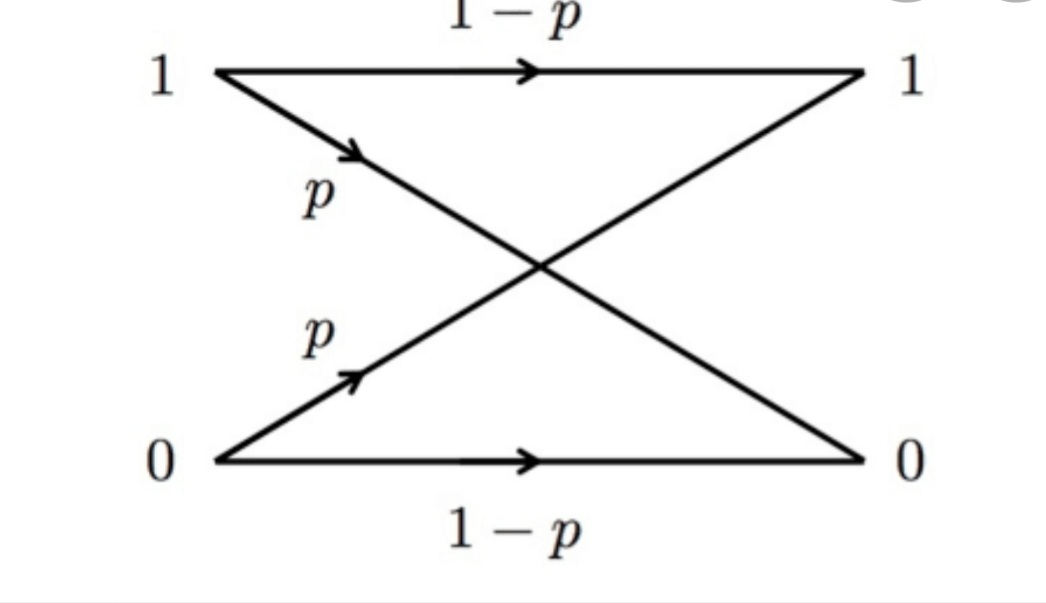
\includegraphics[width=0.5\textwidth]{BSC diagram.jpg}
    \caption{BSC diagram}
\end{figure}
\end{document}